%%
%% This is file `sample-manuscript.tex',
%% generated with the docstrip utility.
%%
%% The original source files were:
%%
%% samples.dtx  (with options: `manuscript')
%%
%% IMPORTANT NOTICE:
%%
%% For the copyright see the source file.
%%
%% Any modified versions of this file must be renamed
%% with new filenames distinct from sample-manuscript.tex.
%%
%% For distribution of the original source see the terms
%% for copying and modification in the file samples.dtx.
%%
%% This generated file may be distributed as long as the
%% original source files, as listed above, are part of the
%% same distribution. (The sources need not necessarily be
%% in the same archive or directory.)
%%
%% The first command in your LaTeX source must be the \documentclass command.
% TODO: Check correct class
\documentclass[sigconf]{acmart}

%% Rights management information.  This information is sent to you
%% when you complete the rights form.  These commands have SAMPLE
%% values in them; it is your responsibility as an author to replace
%% the commands and values with those provided to you when you
%% complete the rights form.

%% TODO: COMPLETE WITH THE ONES GIVEN BY THE CONFERENCE

%% These commands are for a PROCEEDINGS abstract or paper.

%% TODO: COMPLETE WITH THE ONES GIVEN BY THE CONFERENCE

% Add custom packages and commands
\graphicspath{{img/}}
\usepackage{lipsum}   % TODO: Remove once unused
\usepackage{easyReview2}
\usepackage{multirow}
\usepackage{amsmath}
\usepackage{multicol}
\usepackage{balance}
\usepackage{minted}
\setminted[]{
    frame=lines,
    numbersep=5pt,
    breaklines,
    fontsize=\small,
    xleftmargin=.2cm
}

%% Submission ID.
%% Use this when submitting an article to a sponsored event. You'll
%% receive a unique submission ID from the organizers
%% of the event, and this ID should be used as the parameter to this command.
%%\acmSubmissionID{123-A56-BU3}

%%
%% The majority of ACM publications use numbered citations and
%% references.  The command \citestyle{authoryear} switches to the
%% "author year" style.
%%
%% If you are preparing content for an event
%% sponsored by ACM SIGGRAPH, you must use the "author year" style of
%% citations and references.
%% Uncommenting
%% the next command will enable that style.
%%\citestyle{acmauthoryear}

%%
%% end of the preamble, start of the body of the document source.
\begin{document}


% TODO:: Title
%%
%% The "title" command has an optional parameter,
%% allowing the author to define a "short title" to be used in page headers.
\title{Title}


% TODO:: Name
%%
%% The "author" command and its associated commands are used to define
%% the authors and their affiliations.
%% Of note is the shared affiliation of the first two authors, and the
%% "authornote" and "authornotemark" commands
%% used to denote shared contribution to the research.
\author{Author 1}
\email{email.author@one}
\affiliation{%
  \institution{ENSTA Bretagne, Lab-STICC laboratory}
  \city{Brest}
  \country{France}
  \postcode{29200}
}
\author{Author 2}
\email{email.author@two}
\affiliation{%
  \institution{ENSTA Bretagne, Lab-STICC laboratory}
  \city{Brest}
  \country{France}
  \postcode{29200}
}

%%
%% By default, the full list of authors will be used in the page
%% headers. Often, this list is too long, and will overlap
%% other information printed in the page headers. This command allows
%% the author to define a more concise list
%% of authors' names for this purpose.

% TODO:: Name
\renewcommand{\shortauthors}{Name et al.}

%% The abstract is a short summary of the work to be presented in the
%% article.
\begin{abstract}



\end{abstract}


%%
%% The code below is generated by the tool at http://dl.acm.org/ccs.cfm.
%% Please copy and paste the code instead of the example below.
%%
% TODO:: Classification
\begin{CCSXML}
  <ccs2012>
     <concept>
         <concept_id>10011007.10010940.10010941.10010942.10010948</concept_id>
         <concept_desc>Software and its engineering~Virtual machines</concept_desc>
         <concept_significance>500</concept_significance>
         </concept>
     <concept>
         <concept_id>10011007.10011006.10011041.10011044</concept_id>
         <concept_desc>Software and its engineering~Just-in-time compilers</concept_desc>
         <concept_significance>500</concept_significance>
         </concept>
     <concept>
         <concept_id>10010520.10010521.10010522.10010523</concept_id>
         <concept_desc>Computer systems organization~Reduced instruction set computing</concept_desc>
         <concept_significance>500</concept_significance>
         </concept>
   </ccs2012>
\end{CCSXML}
 
\ccsdesc[500]{Software and its engineering~Virtual machines}
\ccsdesc[500]{Software and its engineering~Just-in-time compilers}
% \ccsdesc[500]{Computer systems organization~Reduced instruction set computing}
%%
%% Keywords. The author(s) should pick words that accurately describe
%% the work being presented. Separate the keywords with commas.
\keywords{KW1, KW2}


%%
%% This command processes the author and affiliation and title
%% information and builds the first part of the formatted document.
\maketitle

% ==============================================
% Introduction:
% - Context
% - Presentation of the solution
% - Contributions
% - Sections
% ==============================================

\section{Introduction}

\lipsum[1]

Cite works like \cite{confexample,journalexample,presexample,techreportexample,bookexample}.

% ==============================================
% Background:
% - 
% - 
% - 
% ==============================================

\section{Background - }

\lipsum[3]

\begin{figure}[htbp]
	\centering	
	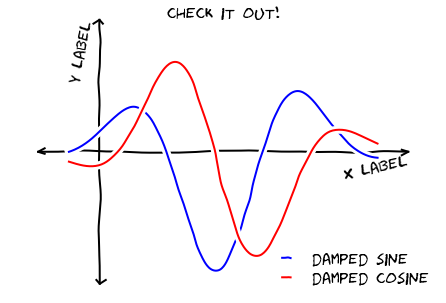
\includegraphics[width=0.48\textwidth]{default.png}
	\caption[Default Small Caption]{Default Caption.}
	\label{fig:DefaultLabel}
\end{figure}

\lipsum[4]

% ==============================================
% Related Works:
% - 
% - 
% - 
% ==============================================

\section{Related Works - }

\lipsum[5]

%           [options] {language}        {file}
\inputminted[linenos]{javascript}{codes/example.js}

% ==============================================
% Solution Design:
% - 
% - 
% -
% ==============================================

\section{Solution Design}

\lipsum[6]

% =========================================================================================
% Gigue parameters
\begin{table}[htbp]
\centering
\begin{tabular}{lll}
\hline
\textbf{Type} & \textbf{Description} & \textbf{Name} \\ \hline
\textit{1} & Param type 1 & \texttt{p1} \\ \hline
\textit{1} & Param type 2 & \texttt{p2} \\ \hline
\textit{1} & Param type 3 & \texttt{p3} \\ \hline
\end{tabular}
\caption{Table name.}
\label{tab:param}
\end{table}
% =========================================================================================

% ==============================================
% Evaluation:
% - 
% - 
% -
% ==============================================

\section{Evaluation}

\subsection{Experimental Setup}

\lipsum[7]

\subsection{Results}

\lipsum[8]

\subsection{Discussion}

\lipsum[9]

% ==============================================
% Conclusion
% - Contrib recap
% - Results recap
% - Future Works
% ==============================================

\section{Conclusion}

\lipsum[10]



%%
%% The acknowledgments section is defined using the "acks" environment
%% (and NOT an unnumbered section). This ensures the proper
%% identification of the section in the article metadata, and the
%% consistent spelling of the heading.
%% \begin{acks}
%% To Robert, for the bagels and explaining CMYK and color spaces.
%% \end{acks}

%%
%% The next two lines define the bibliography style to be used, and
%% the bibliography file.
\balance
\nocite{*}
\bibliographystyle{ACM-Reference-Format}
\bibliography{bibliography}

\end{document}
\endinput
%%
%% End of file `sample-manuscript.tex'.
